%----------------------------------------------------------------------------------------
%	PAQUETES Y OTRAS COSAS DE CONFIGURACION
%----------------------------------------------------------------------------------------
%\documentclass[a4paper,man,natbib,scrbook]{apa6}
\documentclass[12pt]{article}

% esto es una prueba de comment
\usepackage[spanish]{babel}
\usepackage[utf8x]{inputenc}
\usepackage{graphicx}
%\usepackage[colorinlistoftodos]{todonotes} %PAQUETE QUE FALLA JULIO
\usepackage[bottom]{footmisc}
%\usepackage{blindtext} %PAQUETE QUE FALLA JULIO
\usepackage{caption}
\graphicspath{ {images/} }
%\graphicspath{{/home/cursoredes/images/}}
\usepackage{fancyhdr}
\usepackage{enumitem}
\usepackage{hyperref} %INDICE CON VINCULOS
\usepackage{csquotes}

%----------------------------------------------------------------------------------------
%	PAGE HEADERS
%----------------------------------------------------------------------------------------
\setlength{\headheight}{15pt}

\pagestyle{fancy}
\renewcommand{\sectionmark}[1]{ \markright{#1} }

% L=left, R=right, E=even, O=odd

\fancyhf{}
\fancyhead[LE,RO]{\thepage} %Numero pagina
\fancyhead[RE]{\textit{ \nouppercase{\leftmark}} }
\fancyhead[LO]{\textit{ \nouppercase{\rightmark}} }

\fancypagestyle{plain}{ 
  \fancyhf{} 
  \renewcommand{\headrulewidth}{0pt} 
  \renewcommand{\footrulewidth}{0pt}
}
%------------------------------------------------
%
%------------------------------------------------

\begin{document}

\begin{titlepage}

\newcommand{\HRule}{\rule{\linewidth}{0.5mm}} 

\center % Centra todo
 
 
%----------------------------------------------------------------------------------------
%	LOGO SECCION
%----------------------------------------------------------------------------------------

\textsc{\LARGE Universidad Complutense de Madrid}\\[0.1cm] % Universidad

\begin{center}
	\centering
	
\includegraphics[width=0.5\textwidth]{logo}
\end{center}
 
 
%----------------------------------------------------------------------------------------
%	HEADING SECCION
%----------------------------------------------------------------------------------------

\textsc{\LARGE Grupo 4}\\[0.1cm] % Grupo
%\textsc{\Large Heading 1}\\[0.5cm] % Heading mayor
%\textsc{\large Heading 2}\\[0.5cm] % Heading menor

%\textsc{\LARGE Grupo 4}\\[1cm]

%----------------------------------------------------------------------------------------
%	TITULO SECCION
%----------------------------------------------------------------------------------------

\HRule \\[0.4cm]
{ \huge \bfseries HITO 2: FASE DE }\\[0.4cm] % Titulo
{ \huge \bfseries MODELADO Y REQUISITOS}\\[0.2cm] % Titulo
\HRule \\[1.2cm]
 
%----------------------------------------------------------------------------------------
%	AUTHOR SECTION
%----------------------------------------------------------------------------------------

\begin{minipage}{0.4\textwidth}
\begin{flushleft} \large
\emph{Autores:}\\
Ángel \textsc{Cruz} \\ %Nombres
Julio \textsc{de la Cruz} \\
Eduardo \textsc{Alcober}\\
Sergio \textsc{Gómez}\\
Isauro \textsc{López}\\
Darío \textsc{Gallegos}
\end{flushleft}
\end{minipage}
~
\begin{minipage}{0.4\textwidth}
\begin{flushright} \large
\emph{Profesor:} \\
Antonio \textsc{Sánchez} % NOMBRE PROFESOR
\end{flushright}
\end{minipage}\\[0.85cm]

%----------------------------------------------------------------------------------------
%	FECHA SECCION
%----------------------------------------------------------------------------------------

{\large 11 de noviembre de 2018}\\[0.5cm] % Fecha


%----------------------------------------------------------------------------------------
%	CONTENIDO
%----------------------------------------------------------------------------------------

\vfill % Rellenar el resto con espacio en blanco

\end{titlepage}


%\maketitle
%\footnotetext{EJEMPLO DE NOTA A PIE DE PAGINA}

\tableofcontents % Indice de contenidos
\newpage

%----------------------------------------------------------------------------------------
%	INTRODUCCION
%----------------------------------------------------------------------------------------

\section{Introducción}
Apoyándonos en Sinnaps, una aplicación para la gestión de proyectos, de la misma manera que utilizamos en el hito 1, hemos querido distribuir el reparto de tareas para optimizar el tiempo y los recursos disponibles. Las tareas contienen los aspectos más importantes a cumplir, siendo las mismas divididas en subtareas. Detallamos las siguientes con el orden de prioridad correspondiente:

\begin{itemize}

\item \textbf{Documentación}: Permite a todos los miembros de nuestro grupo disponer de las aptitudes y conocimientos necesarios para el siguiente hito.

\item \textbf{Correcciones del hito anterior}: Tras recibir el feedback del anterior hito, es
necesario aplicar las correcciones en general para la entrega final.

\item \textbf{Decisión del modelo a desarrollar}​: El grupo realizó una votación para decidir qué tipo de desarrollo emplearemos, siendo top-down el diseño elegido.

\item \textbf{Procesamiento de datos}: Obtendremos información relevante extraídos durante el análisis de los usuarios.

\item \textbf{Creación de esqueletos}: Nos centramos previamente en identificarlos después de procesar los datos. Hay que dotar a los esqueletos de pseudo-identidad.

\item \textbf{Desarrollo de perfiles}: Para conseguirlo decidimos agrupar toda la información recolectada de la tarea anterior,

\item \textbf{Clasificación del tipo de personas}​: Decidimos explicar los distintos tipos de personas obtenidas en el hito anterior.


\item \textbf{Problemas y visiones}​: Las etapas de investigación y modelado de personas nos permitirán observar de manera más evidente los problemas que nuestros usuarios tienen y desde este punto podemos evaluar las posibles soluciones.

\item \textbf{Lluvia de ideas (brainstorming)}: Tras deliberaciones en grupo obtenemos valoraciones y soluciones a los problemas planteados, tomamos decisiones mientras cada uno aporta lo mejor de sí.


\item \textbf{Identificación de las personas}: Conseguiremos una aproximación al modelo mental del usuario concretamente para las personas primarias y secundarias.


\item \textbf{Creación de escenarios}​: Construiremos las situaciones problemáticas de nuestras personas, y en base ello especificaremos cómo nuestra aplicación puede cubrir las necesidades de éstos tipos de personas.

\item \textbf{Análisis de requisitos}​: Nuestro objetivo es detectar "Qué necesitan" nuestras personas, más allá de lo que podamos pensar nosotros al respecto. Vamos a plantear los requisitos como ternas Acción (a) + Objeto (o) + Contexto (c).


\item \textbf{Generación de artefactos}​: El resultado final de nuestro trabajo en este hito, serán un conjunto de materiales adicionales como los postit que nos permitirán continuar con el siguiente hito. Todavía estamos en una etapa en la que no hemos de descartar nada como imposible en el desarrollo de nuestra aplicación.

\end{itemize}


\begin{center}
	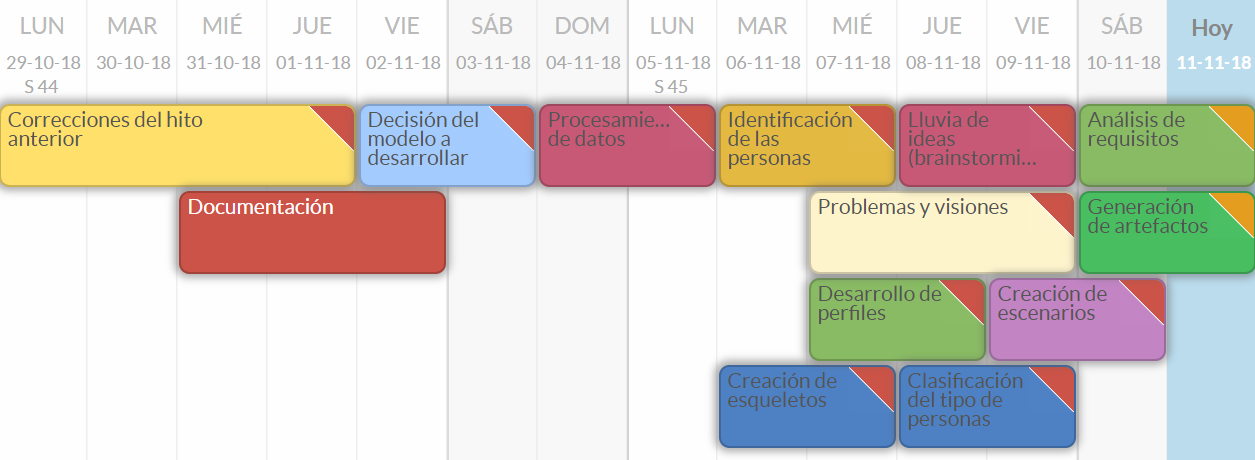
\includegraphics[width=1\textwidth]{planificacionHito2.png}
		\captionof{figure}{Planificación de tareas \href{https://drive.google.com/open?id=1QrF7eOGcyh01kO7jcbpZVWYKA_dWRhWB}{(PDF: planificacionHito2.pdf)} }
\end{center}
\phantom{10}

Este equipo trabaja según el esquema descentralizado controlado\footnote{Organización de equipos según Mantei, Ingeniería del Software}, donde las tareas asignadas a cada miembro podrán ser intercambiadas hacia otro para agilizar el proceso, tratando de ser rápidos ante las incidencias si fuera el caso. Tras la puesta en común de las tareas asignadas, todos los miembros del equipo colaboran activa e individualmente en una o varias revisiones finales de los documentos y artefactos generados.


%----------------------------------------------------------------------------------------
%	MODELADO
%----------------------------------------------------------------------------------------

\section{Modelado}

%----------------------------------------------------------------------------------------
%	TOP DOWN Y CATEGORIA DE USUARIOS.
%----------------------------------------------------------------------------------------
\subsection{Explicación del proceso de diseño top-down}

Para esta fase de diseño de personas hemos decidido utilizar la metodología top-down, pues para la mayoría del equipo le resulta más sencillo partir de especificaciones generales y crear a partir de estas; componentes, categorías, especializar y detallar los requisitos.

\begin{itemize}
\item \underline{Categorías de usuarios}:

Tenemos por el momento dos grandes grupos de usuarios:
\begin{itemize}
\renewcommand{\labelitemi}{$\Rightarrow$}
\item \textbf{Estudiantes}: 

Usuarios que utilizan las instalaciones y hacen reservas sobre el material que dispone la biblioteca.

\item \textbf{Personal de la biblioteca}: 

Usuarios que se encargan de controlar los recursos de la biblioteca.
\end{itemize}

%----------------------------------------------------------------------------------------
%	PROCESADO DE DATOS
%----------------------------------------------------------------------------------------
\subsubsection{Procesado de los datos}

~~~Partiendo de la lista de factoides producida en la etapa anterior, hemos tratado de analizar y encapsular categorías de factoides y factoides en las categorías de usuarios anteriormente mencionadas.

~~~Para realizarlo nos hemos reunido en equipo y pusimos en común aspectos que veíamos reflejados en los factoides obtenidos y lo asignamos a la categoría correspondiente. Hemos representado las categorías de usuarios con pizarras de colores, las categorías de factoides con posits amarillos y en verde clarito los posits que representan factoides concretos.

\begin{center}
	\centering
	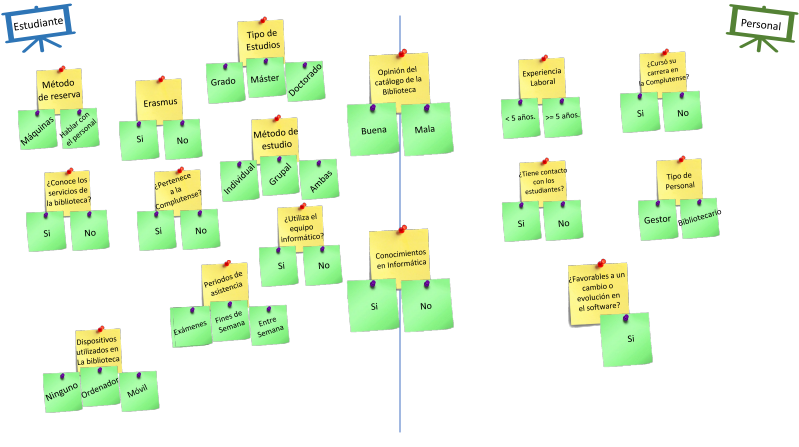
\includegraphics[width=1\textwidth]{fotoPostits}
	\captionof{figure}{Post-its \href{https://drive.google.com/open?id=1G4_21vcZPXV_v715H9-Mw1SJCMis615N}{(PDF: postIts.pdf)}}
\end{center}

%----------------------------------------------------------------------------------------
%	CREACION DE ESQUELETOS
%----------------------------------------------------------------------------------------
\subsubsection{Identificar y crear esqueletos}

~~~Tras procesar los datos hemos identificado tres posibles subgrupos para el grupo de estudiantes y otros dos relacionados con el personal trabajador:
\begin{enumerate}
	\item Estudiantes de la universidad complutense.
	\item Estudiantes que no son de la universidad complutense.
	\item Estudiantes Erasmus.
	\item Bibliotecarios.
	\item Gestores de la Biblioteca.
\end{enumerate}

~~~Para los tres primeros subgrupos se han elaborado los siguientes esqueletos con las características más representativas de cada subgrupo.

\begin{enumerate}
	\item Uso de la biblioteca.
	\item Conocimiento del funcionamiento y servicios de la biblioteca.
	\item Préstamo de material.
	\item Accesibilidad.
\end{enumerate}

~~~Para los bibliotecarios se ha elaborado otro esqueleto con las siguientes características más destacadas.

\begin{enumerate}
	\item Nivel de manejo del Software.
	\item Experiencia.
	\item Contacto con la biblioteca.
\end{enumerate}

\begin{itemize}
	\item \textbf{Estudiante Complutense: }
	\begin{itemize}
	\item \textbf{Nombre(s):}  Alejandro. \\
	\item \textbf{Rago de edad:} 18-26 años. \\
	\item \textbf{Dedicación (profesional si procede):} estudiante. \\
		\item \textbf{Uso de la biblioteca: \\}
			Por lo general se hace un uso individual de las instalaciones y asisten con mucha frecuencia a lo largo del año lectivo. Los usuarios son mayoritariamente estudiantes de grado matriculados en la Universidad Complutense.

			Factoides a partir de los cuales hemos deducido esto: \\--``Los usuarios que trabajan de forma individual en algunos casos pueden llegar a representar el 80\% de los usuarios.''\\ --``El 90 \% de los usuarios estudian un grado/doble grado, el 6.7\% de ellos estudia un máster y el 3.3\% estudian un doctorado.''\\ --``Suelen tener dificultad para encontrar sitio cuando llegan más tarde de lo habitual.''.

		\item \textbf{Conocimiento del funcionamiento y servicios de la biblioteca: \\}
			Al estudiar en la Complutense, en la mayoría de los casos, la asistencia a la María Zambrano va a ser mucho mayor. Esto va a dar un conocimiento mucho mejor sobre los servicios de esta biblioteca y sus procedimientos de uso. Este grupo de usuarios es conocedor de las instalaciones y están familiarizados con ellas.

			Factoides a partir de los cuales hemos deducido esto: \\--``Los usuarios que han valorado positivamente el horario de la biblioteca son usuarios que permanecen largos periodos de tiempo de forma individual en la misma.''.

		\item \textbf{Préstamo de material: \\}
			Pueden reservar libros y equipo informático mostrando el carné de la Universidad Complutense. Por lo general no están contentos con el sistema de reservas actual, ni con la gestión de los puestos en época de exámenes cuando se satura la biblioteca.

			Factoides a partir de los cuales hemos deducido esto: \\--``En exámenes la biblioteca está saturada por lo que suele madrugar para conseguir sitio.'' \\--``Los estudiantes se dejan los carnets para engañar al sistema (por ejemplo en las reservas de libros cuando el carnet propio está bloqueado)'' \\--``Prefiere ser atendido por una máquina en lugar de una persona.''.

		\item \textbf{Accesibilidad: \\}
			La accesibilidad es bastante buena por ser una biblioteca cercana a las facultades y estar bien comunicada. Los usuarios suelen asistir de lunes a viernes con mayor frecuencia que en los fines de semana. En periodos de exámenes la asistencia de estos alumnos puede ser de todo el día, incluso por las noches.

			Factoides a partir de los cuales hemos deducido esto: \\--``Le gusta estudiar de forma individual a lo largo de la semana en la biblioteca y en casa durante los fines de semana.'' \\ --``Estudian prácticamente todo el día.''.

	\end{itemize}
	\item \textbf{Estudiante NO-Complutense:}\\
 En base a los resultados de las encuestas y las entrevistas, no hemos dado con estudiantes de esta categoría, pero pueden existir. Según los servicios de la biblioteca, para acceder en sabado, domingo y festivo y de lunes a viernes a partir de las 21 horas es necesario mostrar el carné ucm o acreditar la pertenencia a la Universidad Complutense de Madrid, pero no fuera de esas franjas. También por su ubicación geográfica (en Ciudad Universitaria) en pleno Campus de la Universidad Complutense y rodeada de sus facultades, es normal que sean estudiantes de  éstas, y no los de otras universidades, aquellos que más abundan, por encima de la pequeña restricción horaria que comentamos. Pero siempre puede acudir alguno para acompañar a algún "estudiante Complutense", luego los vamos a considerar.
	\begin{itemize}
	
		\item \textbf{Nombre(s):}  Francisco. \\
	\item \textbf{Rago de edad:} 18-26 años. \\
	\item \textbf{Dedicación (profesional si procede):} estudiante. \\
	
		\item \textbf{Uso de la biblioteca: \\}
			Estimamos que su asistencia a la biblioteca ocurre en momentos puntuales, como en periodo de exámenes y hacen un uso por lo general individual de la misma. También pueden acudir como acompañantes de un estudiante Complutense.

		\item \textbf{Conocimiento del funcionamiento y servicios de la biblioteca: \\}
			Este grupo de usuarios está poco familiarizado con la biblioteca y por lo general no conocen los servicios que ofrece.

		\item \textbf{Préstamo de material: \\}
			Estos estudiantes no pueden solicitar préstamos.

			Factoides a partir de los cuales hemos deducido esto: \\
			--``Los estudiantes se dejan los carnets para engañar al sistema (por ejemplo en las reservas de libros cuando el carnet propio está bloqueado)'', esto significa que es necesario un carné UCM, al no tener, no pueden reservar.

		\item \textbf{Accesibilidad: \\}
			Este grupo de usuarios no suele encontrarse cerca del campus universitario.

	\end{itemize}
	\item \textbf{Estudiante ERASMUS (Complutense): }
	
	\begin{itemize}
	
		\item \textbf{Nombre(s):}  Mortimer. \\
	\item \textbf{Rago de edad:} 18-26 años. \\
	\item \textbf{Dedicación (profesional si procede):} estudiante. \\
		\item \textbf{Uso de la biblioteca. \\}
			Basándonos en los resultados de la fase anterior, no hemos encontrado a un gran número de estudiantes erasmus, pero podemos asumir que hacen un uso similar de las instalaciones salvo por la reserva y préstamo de material. Además el cambio de lengua puede suponer un obstáculo importante.

			Factoides a partir de los cuales hemos deducido esto: \\--``Tienen problemas para gestionar el carnet de la biblioteca para los estudiantes de Erasmus.'' \\ --``Como estudiante Erasmus le resultaba incómodo tener que rellenar fichas y documentos cada vez que entraba en una biblioteca.''.

		\item \textbf{Conocimiento del funcionamiento y servicios de la biblioteca. \\}
			Son estudiantes que generalmente permanecen poco tiempo en el campus por lo que no llegan a conocer, en muchos casos, todos los servicios que ofrece la biblioteca.

		\item \textbf{Préstamo de material: \\}
			Es complicado para este tipo de estudiante sacar o reservar libros debido a su condición de ERASMUS, en esto también influye el actual software de gestión, que sumado a las trabas del idioma, complica muchas veces que éste tipo de alumnos tengan la posibilidad de obtener préstamos de los materiales de la biblioteca.

			Factoides a partir de los cuales hemos deducido esto: \\ --``Comentan que los estudiantes de Erasmus tienen dificultad para la reserva de libros.'' \\ --``Como estudiante Erasmus le resultaba incómodo tener que rellenar fichas y documentos cada vez que entraba en una biblioteca.''.

		\item \textbf{Accesibilidad: \\}
			Disponen de la misma accesibilidad que los estudiantes de la Complutense.

	\end{itemize}
	\item \textbf{Personal Bibliotecario: }
	\begin{itemize}
		\item \textbf{Nivel de manejo del Software: \\}
			Son usuarios expertos de los sistemas informáticos de la biblioteca, conocen todas sus funcionalidades y su trabajo consiste en explicárselo a los diferentes usuarios que acuden a esta.
			
		\item \textbf{Experiencia: \\}
			La experiencia de estos usuarios es variada, generalmente acomodándose en los extremos, llegando a abarcar desde becarios novatos hasta longevos trabajadores con décadas de experiencia.
			
		\item \textbf{Contacto con la biblioteca: \\}
			Trabajan todo el dia de cara al público, ayudando a los estudiantes con los diferentes servicios que ofrece la biblioteca. Los bibliotecarios son el escalón más bajo en la jerarquía de la biblioteca.
			
			Factoides a partir de los cuales hemos deducido esto: \\ --``En la experiencia de Maria los estudiantes nos solicitan salas de trabajo en grupo reducidas (de 6 a 8 personas)'' \\ --``Maria dice que hay poco personal en la Maria Zambrano para controlar a tantas personas''.
			\newpage
			
	\end{itemize}
	\item \textbf{Personal Gestor: }
	\begin{itemize}
		\item \textbf{Nivel de manejo del Software: \\}
			Son los responsables de probar y decidir si determinado software se puede o no implantar en la gestión de la biblioteca. No tienen un contacto diario con los programas, pero los conocen bien. Deciden los horarios y los trabajadores de la biblioteca, así como la implantación de nuevos sistemas (ej. tornos, lectores de tarjeta id… esta información está extraída de una conversación previa a la entrevista).
			
		\item \textbf{Experiencia: \\}
			Más de 5 años trabajando en la gestión de la Biblioteca le proveen de un conocimiento profundo de su funcionamiento complementado por su labor de toma de decisiones.
			
		\item \textbf{Contacto con la biblioteca: \\}
			Es un trabajador gestor de la biblioteca, que está menos en contacto ``físico'' con la biblioteca y estudiantes, pero que tiene un punto de vista y un conocimiento completo ``desde fuera'' tanto de la infraestructura como del funcionamiento de la biblioteca, ya que se dedica a su gestión. Los gestores están un nivel más arriba en la jerarquía de control de la biblioteca.
			
	\end{itemize}
\end{itemize}

%----------------------------------------------------------------------------------------
%	PRIORIZAR ESQUELETOS
%----------------------------------------------------------------------------------------
\subsubsection{Priorizar los esqueletos}
\begin{itemize}
	\item \textbf{Estudiante Complutense:}
		Por estadística, la persona más frecuente y común es el estudiante de la universidad complutense, por ello este tipo de persona es crítica y fundamental en el desarrollo de nuestro sistema.
		A continuación se encuentran los estudiantes Erasmus que representan el siguiente grupo de personas mas frecuentes y con mayores necesidades, finalmente se encuentran las personas que no pertenecen a la complutense.

	\item \textbf{Personal Bibliotecario:}
		Hemos decidido sintetizar los dos perfiles de trabajadores de la biblioteca, ``gestor'' y ``bibliotecario'' como ``personal bibliotecario'' con vistas a unificar la información de la que disponemos y simplificar la jerarquía. Esta va a ser nuestra persona secundaria, que además del front-end de la aplicación, utilizará la parte de back-end para su gestión.

\end{itemize}

\newpage
%----------------------------------------------------------------------------------------
%	PERSONAS
%----------------------------------------------------------------------------------------
\subsubsection{Desarrollar las personas a partir de los esqueletos}

\begin{center}
	\centering
	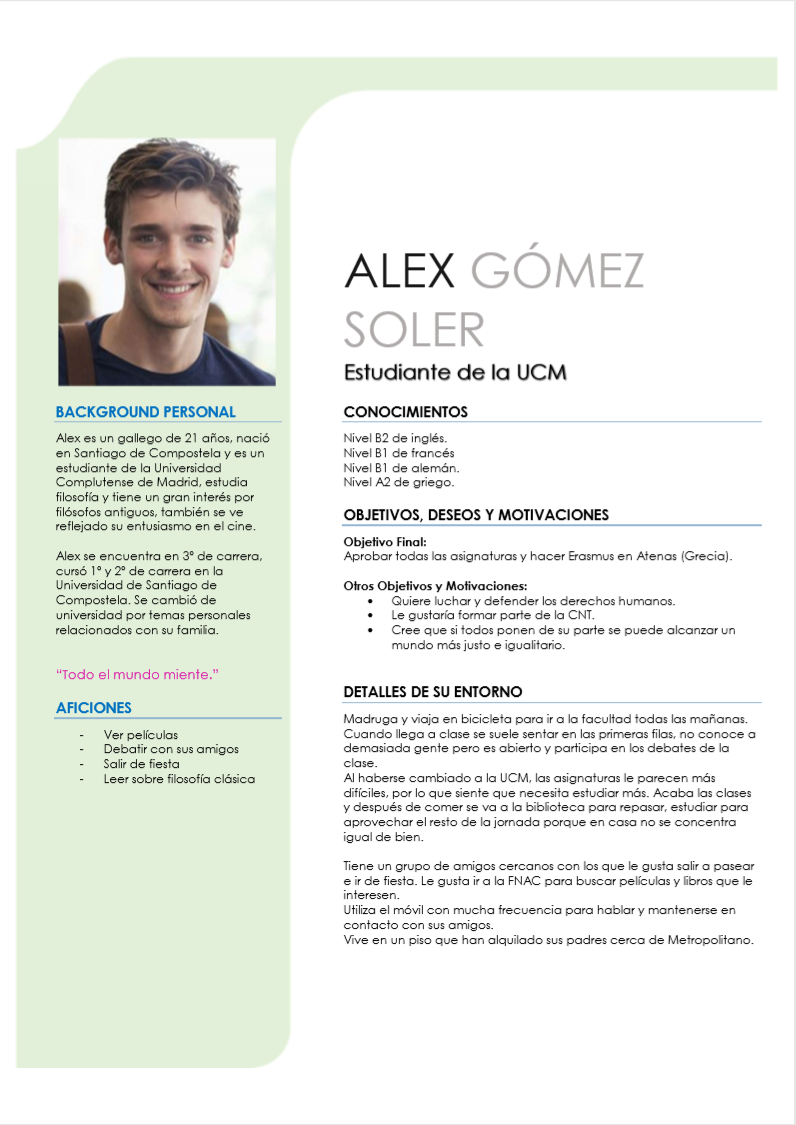
\includegraphics[width=0.9\textwidth]{fotoAlex}
	\captionof{figure}{Ficha de estudiante Complutense \href{https://drive.google.com/open?id=1wAC7VK-p0av5COayJL5kajCv9lOpeVVq}{(PDF: fichaAlex.pdf)}}
\end{center}

\begin{center}
	\centering
	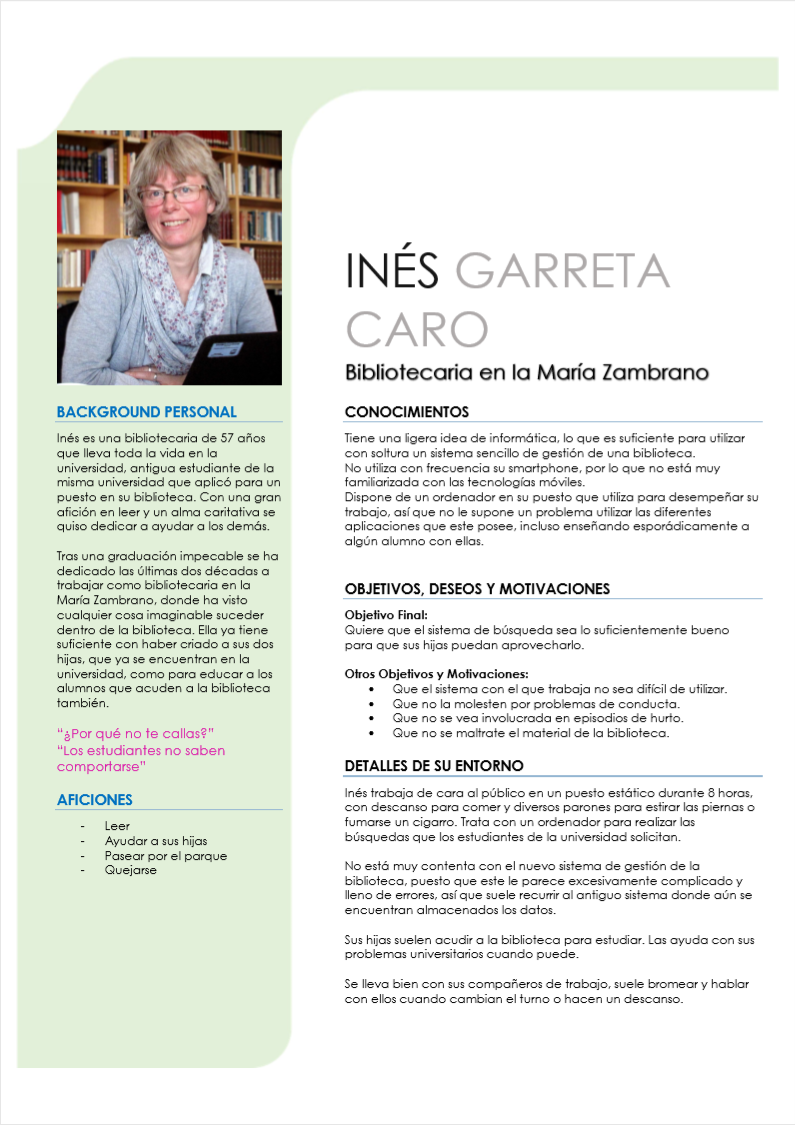
\includegraphics[width=0.90\textwidth]{fotoInes}
	\captionof{figure}{Ficha de bibliotecaria \href{https://drive.google.com/open?id=1mq0vCbA2Y4_7YjZU8RLorK9UxO5XRayi}{(PDF: fichaInes.pdf)}}
\end{center}

\newpage
%----------------------------------------------------------------------------------------
%	VALIDACION Y TIPOS DE PERSONA
%----------------------------------------------------------------------------------------
\subsection{Explicación de tipos de Persona}

~~~A partir de lo anterior, hemos clasificado a estas personas en los siguientes tipos:

\begin{itemize}
	\item \textbf{Personas primarias}: \\
		Nuestra persona primaria es Alex, estudiante de la UCM. Representa a los usuarios principales de la aplicación. Para esta persona diseñaremos la interfaz principal con sus funciones correspondientes. El objetivo es cubrir sus necesidades.
	
	\item \textbf{Personas secundarias}: \\
		Nuestra persona secundaria es Inés, representan al personal de la biblioteca. La mayoría de las necesidades de Inés están cubiertas con la interfaz principal de Alex, pero además requieren de alguna funcionalidad extra, relacionadas por ejemplo con la información del inventario de los materiales de la biblioteca.
		
	\item \textbf{Personas suplementarias}: \\
		Nuestras personas suplementarias son los estudiantes de Erasmus, docentes y el gestor de la biblioteca. Sus necesidades quedan cubiertas por las interfaces de los tipos de personas anteriormente mencionadas. No necesitan ninguna funcionalidad extra.

	\item \textbf{Personas negativas o antipersonas}: \\
		Son personas que no van a usar la aplicación. Hemos reconocido como parte de esta categoría a  estudiantes de la UCM que deciden no ir a la biblioteca ,estudiantes de otras universidades, estudiantes de selectividad y particulares. 
		
\end{itemize}
\end{itemize}

\newpage
%----------------------------------------------------------------------------------------
%	REQUISITOS
%----------------------------------------------------------------------------------------
\section{Requisitos}
\subsection{Enunciado de problemas y visiones}
\begin{enumerate}

\item \textbf{Problema:} En época de exámenes es difícil encontrar sitio a medio día y por la tarde. \\
\textbf{Visión:} Nuestra aplicación permitirá reservar sitio en la biblioteca para asegurar que el usuario dispone de una plaza cuando llegue.

\item \textbf{Problema:} Durante los días donde hay mucho flujo de personas es muy difícil contar cuántas están dentro, dificultando saber si se ha llegado al aforo completo. \\
\textbf{Visión:} Nuestra aplicación registrará el número de mesas/sitios que estén reservadas sabiendo así el número de sitios libres u ocupados.

\item \textbf{Problema:} Largas colas en la maquina de reservas para reservar o tomar prestados libros. \\
\textbf{Visión:} Nuestra aplicación permitirá hacer la reserva de un libro sin necesidad de pasar por la máquina, agilizando este proceso.

\item \textbf{Problema:} Buscar el libro deseado puede conllevar tiempo, aún solicitando la ayuda de una bibliotecaria. \\
\textbf{Visión:} Nuestra aplicación permite localizar con un mapa el lugar en el que se encuentra el libro y saber si existen unidades disponibles.

\item \textbf{Problema:} Solicitar equipo informático a una bibliotecaria hace que esta tenga que comprobar si quedan unidades disponibles y en ese caso, registrar el préstamo. \\
\textbf{Visión:} Con nuestra aplicación el estudiante puede saber si existen unidades de ese equipo informático que quiera solicitar. Permitirá registrar su préstamo para que cuando solicite el material a la bibliotecaria, esta vea en su ordenador que dicho estudiante lo ha reservado, y facilitará a la bibliotecaria el registro de este material al estudiante.

\item \textbf{Problema:} Gente nueva o que desconoce la biblioteca puede tener dificultades para llegar hasta ella, además los estudiantes pueden no conocer el horario y, consecuentemente, no aprovecharlo. \\
\textbf{Visión:} Nuestra aplicación contendrá la información general (dirección, horario, transporte, ...) de la biblioteca, facilitando así que el usuario acceda y disponga de ella.

\end{enumerate}
\subsection{Lluvia de ideas (brainstorming)}

\begin{itemize}[noitemsep]

\item Aplicación para móvil.

\item Aplicación Open Source.

\item Interfaz sencilla.

\item Registro de códigos QR de sitios/mesas por la cámara del móvil.

\item Modo día/noche.

\item Filtros del motor de búsqueda: Año, Autor, Título, Tema(s), Lengua, Género...

\item Posibilidad de seleccionar una asiento para reservar buscándolo en el mapa.

\item Ver el estado actual de la biblioteca y ver qué asientos están disponibles.

\item Tras realizar una búsqueda aparece una lista de resultados relacionados.

\item Registro en la app con el email de la UCM.

\item Visualización de un mapa de la María Zambrano con la localización de los libros.

\item Notificaciones vía correo UCM sobre retrasos que se puedan realizar.

\item Muestra el calendario con los días y el horario de la biblioteca.

\item Muestra un mapa de dónde se situa y cómo se puede llegar a ella.

\item Muestra un menu de reserva de materiales informáticos.

\end{itemize}

%-------------------------------------------------------------------------------------------
% EXPEXTATIVAS DE PERSONAS
%-------------------------------------------------------------------------------------------
\subsection{Identificación de las expectativas de las personas}
\begin{itemize}[noitemsep]

\item \textbf{Alex (persona primaria - estudiante de la Complutense)} \\
Está estudiando Filosofía. Quiere aprobar todas las asignaturas para poder ir de Erasmus a Atenas, la cuna de la democracia. Es un estudiante aplicado, al que le gustaría formar parte del CNT. Le preocupa  la desigualdad que existe y cree que si todos ponen de su parte se puede alcanzar un mundo más justo.
Se acaba de cambiar  a la UCM y todo es nuevo para él. Las asignaturas le parecen más complicadas que las de su antigua universidad, por lo que después de comer suele ir directo a la biblioteca a estudiar.\\

Normalmente la biblioteca no está llena, pero hay días en los que casi imposible encontrar sitio ya que todos los  sitios están ocupados, y no por que haya un alumno sentado sino porque esta lleno de hojas o libros a modo de guardar el puesto. No le parece justo que la gente se vaya y deje sus cosas ahí. Alex quiere saber que puestos están libres y cuáles no, y en caso de estar ocupado durante cuánto tiempo. De la misma manera, le gustaría saber donde están los puestos libres ya que al ser tan grande la biblioteca, pierde mucho tiempo recorriendola .\\

A Alex le encanta leer sobre todo filosofía clásica y le gustaría encontrar los libros por sí solo pero le resulta complicado usar CISNE (el buscador de la biblioteca ) y acaba pidiendo ayuda a los bibliotecarios. También le gustaría poder mirar si el libro está disponible y si no lo esta, que le enviasen una notificación el mismo día que sea devuelto. Si un libro le parece interesante quiere poder guardarlo en favoritos, y si tiene varios libros guardados poder distinguirlos por categorías o autores.\\

Está muy conectado a la redes sociales y siempre lleva el móvil encima por lo que le gustaría que la aplicación sea para dispositivo móvil.\\

\item \textbf{Inés (persona secundaria - personal de la biblioteca)} \\
	Trabaja como bibliotecaria de la UCM, lleva toda la vida en la universidad. Antigua estudiante de la misma que decidió opositar para el puesto de bibliotecaria. Mujer con carácter, con una gran afición por la lectura que ama su trabajo y ayudar a los demás. Tiene dos hijas que estudian en la universidad por lo que le gustaría que el sistema sea lo suficientemente bueno como para que sus hijas aprovechen la biblioteca al máximo.\\

Al trabajar tantos años en la biblioteca, la conoce como la palma de su mano y sabe lo que funciona y lo que. Le gustaría que el sistema de CISNE sea más fiable pues de vez en cuando falla  y debe recurrir al antiguo sistema de gestión . Tiene una ligera idea de informática, lo que le permite trabajar en entornos sencillos, pero el nuevo sistema le parece muy complicado por lo que le gustaría uno más sencillo e intuitivo.\\

Le gustaría tener un tablón de tareas para organizarse mejor y que le avisen si por casualidad se le olvida hacer algo. De momento lleva el control apuntando en un  agenda o en papeles, pero a veces se pierden sus notas. En caso de ser una tarea en común le gustaría poder hablar con ellos para organizar el trabajo, dividir la tarea y asegúrese así que todos están informados de lo que hay que hacer.\\

\end{itemize}

\subsection{Construcción de los escenarios de contexto}
\begin{itemize}[noitemsep]

\item \textbf{Alex (persona primaria - estudiante de la Complutense)} \\
Sus clases en la facultad de Filosofía empiezan a primera hora, por ello todas las mañanas va en bicicleta a su facultad, no suele tardar más de 20 minutos.\\ 

En una asignatura que ha tenido hoy se han enfocado en la filosofía moderna. A él más le llama la atención todo lo relacionado a la filosofía clásica, pero se ha dado cuenta de lo interesante que puede llegar a ser éste otro género.\\

Tiene pensado hoy estudiar y buscar en la biblioteca, algún libro relacionado con la filosofía moderna para ampliar sus conocimientos sobre lo que ha estudiado en clase.
Durante el receso que hay entre una clase y otra, abre la aplicación con el objetivo de reservar sitio y el libro deseado guiándose por el argumento y la valoración media, y así asegurar que dispondrá de una plaza y del libro ya que suele ir a la biblioteca después de comer en la facultad. Él sabe que en época de exámenes es difícil encontrar sitio y libros disponibles a medio día y por la tarde.\\

Después de buscar un poco encuentra los apartados relacionados a los sitios y libros, y dentro de cada uno de ellos las opciones de reserva y en el caso de los sitios también la ubicación de los mismos, además también cuentan con apartados para comentar y valorar  dichos servicios.\\
	
Tras acabar el primer capítulo y quedar convencido del libro, procede a abrir la aplicación para participar en los comentarios y valoraciones. Además decide seleccionar el libro como favorito y seguir a algunos usuarios que comentan de forma muy similar a él.\\

Después, consulta su perfil en el que ve, entre otras cosas, que este libro ya le sale entre su selecta lista de libros destacados y también, en la lista de perfiles seguidos, los
nombres de los dos usuarios a los que acaba de seguir.\\

Consultando después la agenda de los horarios en la aplicación, Alex se fija que la aplicación incorpora un sistema de notificaciones. Tiene varias: los nuevos libros retirados, con la fecha de devolución, mesas y sitios disponibles que seleccionó con el objetivo de que se le avisará cuando se encuentren libres y tiene una solicitud de chat de su amigo Paco. Antes de continuar revisando más a fondo la aplicación decide editar su perfil cambiando la imagen que viene por defecto y algunos datos añadidos cuando creó su cuenta.\\

\item \textbf{Inés (persona secundaria - personal de la biblioteca)} \\
Se despide de su familia muy temprano porque hoy le ha tocado trabajar de mañana, luego se dirige a coger su coche e intentar evitar el atasco rutinario semanal. Sabe que tiene un largo día de trabajo por delante, ya que su jornada empieza a las 09:00 y en el periodo de exámenes entre sus compañeros se distribuyen sus horarios donde hay días que a Inés le tocará trabajar por la mañana, tarde o noche.\\

Entre sus compañeros suelen comentar sobre la nueva aplicación que les ayuda a realizar su trabajo de forma más eficiente y de forma intuitiva, con ello cuentan con más tiempo para organizar físicamente el inventario entre otras cosas.\\

En los momentos de menos afluencia de estudiantes, aprovecha en consultar la aplicación en su móvil, lo primero que visualiza son las notificaciones relacionadas a las entregas de los libros prestados, libros reservados, libros sin ejemplares disponibles, aforo completo respecto a sitios y mesas, tareas que no ha realizado en el horario preestablecido.\\

Después aprovecha en marcar desde la aplicación las tareas realizadas por ella y por supuesto esto le ayuda a gestionar mejor su tiempo sabiendo que tareas le queda pendiente de completar durante su jornada laboral. Además en caso de ser una tarea en común, dichas tareas son distribuidas como subtareas para que cada uno de los integrantes en todo momento pueda saber a quién le queda por completar su trabajo.\\
	
Inés antes de terminar su jornada laboral, abre la aplicación nuevamente para visualizar el estado de sus tareas o subtareas asignadas y si fuera el caso; informar a sus compañeros de cuales no ha podido concluir si las mismas requiriesen ser finalizadas ese mismo día, para que los compañeros del siguiente turno puedan tomar una decisión y solventar dicho problema.\\

\end{itemize}

%------------------------------------------------------------------------------------------------------------
%               3.5 IDENTIFICACION DE LOS REQUISITOS
%------------------------------------------------------------------------------------------------------------
\subsection{Identificación de requisitos}

%-----------------Requisitos de datos---------------------------------
\subsubsection{Requisitos de datos}
\begin{itemize}[noitemsep] 
\item Representación de ejemplar Calendario. Cada usuario puede configurar cinco calendarios. 
\item Ejemplar Tarea.
\item Listas de Tareas (filtrable).
\item Avisos ligados a tareas.
\item Listado de eventos donde poder filtrar (por estado, fecha…) para consultar su estatus. Necesaria jerarquía de usuarios para el acceso versión bibliotecario (Jefes equipo / Personal Biblioteca).
\item Representación de los puestos disponibles en las salas de la biblioteca según sus servicios disponibles y las franjas de tiempo de uso. También se gestiona una lista de puestos favoritos.
\item Representación de mapas conceptuales de los puestos con su código y estado.
\item Perfil de puesto de estudio, que incluye servicios, estado. En caso de estar ocupado muestra la hora que se quedará libre.
\item Ficha de libros de catálogo tiene una interacción con programación de avisos si el libro seleccionado está ocupado. 
\item Un usuario puede marcar como favorito un libro lo que incrementa el contador de favoritos y se añade a lista favoritos del usuario
\item En el perfil personal existe: una imagen, descripción, contacto, followers y following, estadísticas e información institucional
\end{itemize}
%-----------------Requisitos de funcionales------------------------------
\subsubsection{Requisitos funcionales}
\begin{itemize}[noitemsep]
\item Incorporar una función de calendario/agenda. que permita programar eventos y avisos.
\item Además de los eventos añadidos por el usuario, se añadirán automáticamente los límites de estancia cuando se reserve un puesto, la hora de devolver determinado equipo informático o la fecha de devolución del ejemplar solicitado en la biblioteca.
\item Se podrá invitar a otros usuarios de la aplicación y avisarlos conjuntamente cuando venza el evento al que se inscriban, previa confirmación.
\item Calendario tiene las funciones de importar archivo calendario, nuevo calendario, eliminar calendario, fusionar calendario. En él hay tareas como añadir tarea, eliminar tarea, listar tareas por día, listar tareas por mes, añadir participantes (por admin de equipo de bibliotecarios/un estudiante puede añadir otros estudiantes) allí hay una ficha tarea que permite programar avisos, cambiar nombre y cambiar horas
\item La aplicación muestra un mapa, accesible  por salas, de los puestos libres y ocupados, actualizado en cada consulta.
\item Puedes pedirle al sistema que te avise mediante email o notificación cuando se quede libre determinado puesto.
\item Asientos distribuidos por sala en un área tienen un perfil de puesto (ej 232-C, el número de asiento) con unos servicios como marcar favorito, comentario de otros usuarios y opc. valorar, y unas prestaciones como el nº de enchufes o si tiene ordenador
\item Hace la reserva de libros, muestra todos los ejemplares idénticos y en qué biblioteca se encuentran y los organiza por disponibilidad.
\item Puedes pedirle al sistema que te avise mediante email o notificación cuando se devuelva el libro para poder hacer la reserva. 
\item Comprobar si el libro al que se le quiere hacer la reserva (y todos los libros con el mismo nombre) está disponible, si no lo está, indica la fecha en la que tiene que ser devuelto y el estado de devolución de este (por si no lo devuelven a tiempo)
\item Si activas el aviso, el libro se “pre-reserva” durante 1 día para que el usuario que lo devuelva no pueda reservarlo de nuevo justo en ese momento.
\item Notificaciones de la app: puestos de estudio, solicitudes de chat, nuevo follower, respuestas a comentarios y avisos de puestos
\item Notificaciones bibliotecario: Entrega de libro caducada, libro sin ejemplares disponibles, aforo completo, libros reservados y tareas inconclusas (Estas son notificaciones extras por tipo de usuario)
\item Poder organizar los libros de la búsqueda y del apartado “favoritos” por categorías y autores, así como añadir o eliminar nuevos libros a favoritos.
\item En la biblioteca hay un buscador que encuentra los perfiles de los libros seleccionados y  tiene las opciones de reservar, marcar favorito y ver comentarios de otros usuarios con enlace a sus perfiles con la posibilidad de follow o valoración de 1 a 5 estrellas
\item Enlazado al perfil personal del estudiante está el apartado “favoritos” donde el usuario puede gestionar esta lista de forma privada
\end{itemize}

%-----------------Requisitos de contexto------------------------------
\subsubsection{Requisitos de contexto}
\begin{itemize}[noitemsep]
\item Esta funcionalidad ha de estar implementada tanto en la versión de escritorio como en la de móvil.
\item Simplificar la interfaz de la versión móvil respecto a la de escritorio para facilitar la comprensión de los procesos a usuarios menos avanzados, o que utilizan la aplicación “en movimiento” mientras se desplazan de un sitio a otro.
\item No se podrá reservar un puesto si la cuenta con la que se realiza la reserva está sancionada.
\item No se podrá reservar más de un puesto con una única cuenta. Sin embargo se pueden reservar mas entregando el id del resto de cuentas. Si los dueños de estas cuentas no aparecen se les sancionara la cuenta. Si los dueños afirman no haber dado permiso para que su cuenta se utilice para la reserva de dichos puestos se investigará el caso y se procederá a jurisdicción de los empleados (de seguridad o los bibliotecarios).
\item No se podrá reservar un libro más de 3 veces (45 días) y no se podrá reservar el mismo libro inmediatamente después de la devolución si otro estudiante también quiere reservarlo.
\end{itemize}

\end{document}

%COMENTAARIOS
% \todo[inline, color=green!40]{EJEMPLO DE COMENTARIO}

% PARA INCLUIR UNA FOTOGRAFIA:
%\begin{figure}
%\centering
%\includegraphics[width=0.5\textwidth]{~/DIRECCION/A/IMAGEN.jpg}
%\caption{\label{fig:imagen}DESCRIPCION.}
%\end{figure}

% \dots

% ENUMERACION:
%\begin{enumerate}
%\item Enumeracion 1
%\item Enumeracion 2
%\end{enumerate}

%\begin{itemize}
%\item PUNTO 1

% PARA INCLUIR UNA TABLA:
%\begin{table}[h] %LA h PARA INDICAR QUE LA TABLA NO SEA FLOATING
%\centering
%\begin{tabular}{l|r}
%Fila 0 \\\hline
%Fila 1 & Contenido 1 \\
%Fila 2 & Contenido 2
%\end{tabular}
%\caption{\label{tab:widgets}Ejemplo de tabla.}
%\end{table}

%\item PUNTO 2
%\end{itemize}

%\bibliography{BIBLIOGRAFIA}


